%
% ####################################################################################################################################################################################
% ####################################################################################################################################################################################
% ####################################################################################################################################################################################
% ####################################################################################################################################################################################
%

\documentclass[]{myHOWTO-V001}

%
% ####################################################################################################################################################################################
% ####################################################################################################################################################################################
%

\usepackage{myTCB-V001}

%
% ####################################################################################################################################################################################
% ####################################################################################################################################################################################
%

\title{The \textbf{myTCB-V1} Package\\{\small Tables}}
\version{1.00}
\author{Norbert EHART (norbert@ehart.net)}
\date{\today}

%
% ####################################################################################################################################################################################
% ####################################################################################################################################################################################
% ####################################################################################################################################################################################
% ####################################################################################################################################################################################
%

\begin{document}
	
%
% ####################################################################################################################################################################################
% ####################################################################################################################################################################################
%

\selectlanguage{english}

%
% ####################################################################################################################################################################################
% ####################################################################################################################################################################################
%

\maketitle

%
% ####################################################################################################################################################################################
% ####################################################################################################################################################################################
%

\tableofcontents

%
% ####################################################################################################################################################################################
% ####################################################################################################################################################################################
%

\section{Introduction}

\LaTeX{} is mainly used in scientific fields such as electrical engineering, mechanical engineering and computer science. Especially in these fields it is sometimes necessary to create tables.

\qquad
\begin{myFIG}{}
\begin{myTABlst}{TITLE1}{tabularx={C|C|C|C|C}, width=8cm}
	& one     & two     & three    & four     \\
	\hline
	red   											& 1000.00 & 2000.00 & 3000.00  & 4000.00  \\
	\hline
	green 											& 2000.00 & 3000.00 & 4000.00  & 5000.00  \\
	\hline
	blue  											& 3000.00 & 4000.00 & 5000.00  & 6000.00  \\
	\hline
	\textbf{sum}   											& \textbf{6000.00} & \textbf{9000.00} & \textbf{12000.00} & \textbf{15000.00}
\end{myTABlst}
\end{myFIG}

The \emph{myTCB-V1} package provides an environment for this.

The \emph{myTCB-V1} package loads automatically the packages shown in \styref{loadingpackages}.

\begin{mySTYdoclst}{Packages}{label={sty:loadingpackages}}
\RequirePackage{lipsum}

\RequirePackage{graphicx}
\RequirePackage{wrapfig}

\RequirePackage{xcolor}

\RequirePackage{tabularx}
\RequirePackage{colortbl}
\RequirePackage{multirow}

\RequirePackage{verbatim}
\RequirePackage{fancyvrb}
\RequirePackage{listings}

\RequirePackage{float}

\RequirePackage{refstyle}

\RequirePackage{tcolorbox}
	\tcbuselibrary{skins,breakable,listings,xparse}
\end{mySTYdoclst}

To load the package, write \Verb|\usepackage{myTCB-V1}| in the preamble of your document. To use this package, it is highly recommended to have the complete \LaTeX{} distribution installed. This will avoid problems with dependencies.

\begin{myTEXEXdoclst}{Loading myTCB-V1}{label={texex:loadingmyTCBv1}}
\usepackage{myTCB-V1}
\end{myTEXEXdoclst}

%
% ####################################################################################################################################################################################
% ####################################################################################################################################################################################
%

\section{The Table Environment without a List Index}

The \emph{myTCB-V1} package has a predefined environment, which is called \Verb|myTAB|. In this environment there is no list index available and only tables are created

\begin{myTEXEXdoclst}{}{listing and text, listing options={escapechar=\!}}
\begin{myTAB}{tabularx={C|C|C|C|C}, width=8cm}
									& one     					& two     				 & three    				 & four 						\\
	\hline
	red   					& 1000 							& 2000 						 & 3000  						 & 4000  						\\
	\hline
	green 					& 2000 							& 3000 						 & 4000  						 & 5000  						\\
	\hline
	blue  					& 3000 							& 4000 						 & 5000  						 & 6000  						\\
	\hline
	\textbf{sum}   	& \textbf{6000} 		& \textbf{9000} 	& \textbf{12000} 	& \textbf{15000}
\end{myTAB}
\end{myTEXEXdoclst}

A title can be submitted as an optional argument, which appears on the bottom of the table.

\begin{myTEXEXdoclst}{}{listing and text, listing options={escapechar=\!}}
\begin{myTAB}{tabularx={C|C|C|C|C}, title={myTABLE}, width=8cm}
									& one     					& two     				 & three    				 & four 						\\
	\hline
	red   					& 1000 							& 2000 						 & 3000  						 & 4000  						\\
	\hline
	green 					& 2000 							& 3000 						 & 4000  						 & 5000  						\\
	\hline
	blue  					& 3000 							& 4000 						 & 5000  						 & 6000  						\\
	\hline
	\textbf{sum}   	& \textbf{6000} 		& \textbf{9000} 	& \textbf{12000} 	& \textbf{15000}
\end{myTAB}
\end{myTEXEXdoclst}

You can even put a table into a box.

\begin{myTEXEXdoclst}{}{listing and text, listing options={escapechar=\!}}
\begin{myFIG}{}
	\begin{myTAB}{tabularx={C|C|C|C|C}, title={myTABLE}, width=8cm}
									& one     					& two     				 & three    				 & four 						\\
	\hline
	red   					& 1000 							& 2000 						 & 3000  						 & 4000  						\\
	\hline
	green 					& 2000 							& 3000 						 & 4000  						 & 5000  						\\
	\hline
	blue  					& 3000 							& 4000 						 & 5000  						 & 6000  						\\
	\hline
	\textbf{sum}   	& \textbf{6000} 		& \textbf{9000} 	& \textbf{12000} 	& \textbf{15000}
	\end{myTAB}
\end{myFIG}
\end{myTEXEXdoclst}



%
% ####################################################################################################################################################################################
% ####################################################################################################################################################################################
%

\section{The Table Environment with a List Index}

The \emph{myTCB-V1} package has a predefined environment, which is called \Verb|myTABlst|. In this environment there is a list index available and only tables are created. A title (\verb|TITLE1|) must be passed as a mandatory argument. This title does not appear on the box, instead it is found in the list index. The box itself is titled with \emph{Table} and a sequential number.

\begin{myTEXEXdoclst}{}{listing and text, listing options={escapechar=\!}}
\begin{myFIG}{}
	\begin{myTABlst}{TABLE001}{tabularx={C|C|C|C|C}, width=8cm}
									& one     					& two     				 & three    				 & four 						\\
	\hline
	red   					& 1000 							& 2000 						 & 3000  						 & 4000  						\\
	\hline
	green 					& 2000 							& 3000 						 & 4000  						 & 5000  						\\
	\hline
	blue  					& 3000 							& 4000 						 & 5000  						 & 6000  						\\
	\hline
	\textbf{sum}   	& \textbf{6000} 		& \textbf{9000} 	& \textbf{12000} 	& \textbf{15000}
	\end{myTABlst}
\end{myFIG}
\end{myTEXEXdoclst}

\begin{minipage}{0.46\linewidth}
\centering
\begin{myFIGlst}{}{label={fig:mytablofdef}}
	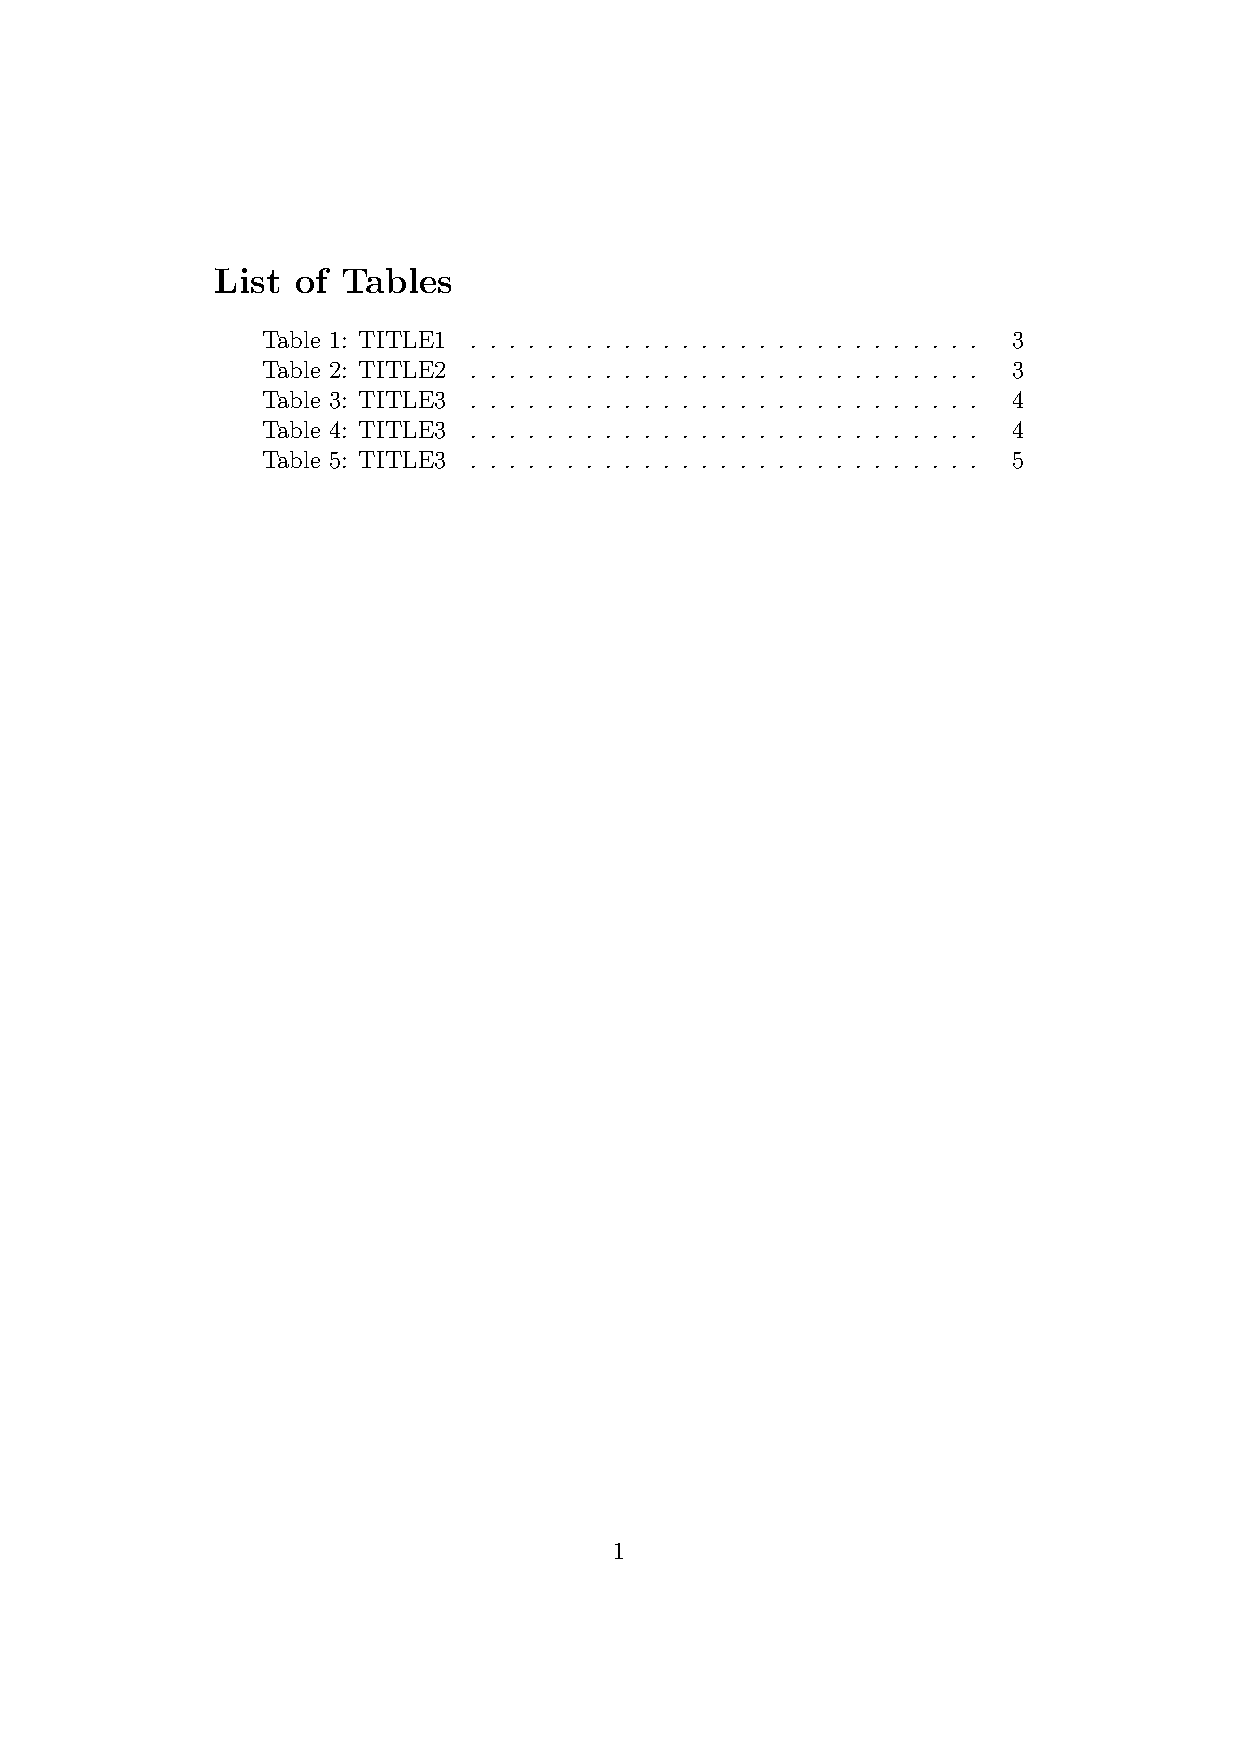
\includegraphics[page=1,scale=0.18]{examples/myTABV000.pdf}
\end{myFIGlst}
\end{minipage}
\begin{minipage}{0.46\linewidth}
You can create the list index with the command \Verb|\listofmyTAB|.

\begin{myTEXEXdoclst}{List Entries of MySTY}{label={texex:mystylistentry}, listing only}
\listofmyTAB
\end{myTEXEXdoclst}

This will create a list index which looks like the picture in \figref{mytablofdef}. 
\end{minipage}

If you want to change the horizontal spacing of the list entries, you can do this quite simple with the following code in the preamble, which is illustrated in \texexref{remleadnumbmytab}.

\begin{myTEXEXdoclst}{Altering the List Index Spacing of myBOXlst}{label={texex:remleadnumbmytab}, listing only}
\makeatletter
	\renewcommand{\l@myTAB}{\@dottedtocline{1}{0mm}{0mm}}
\makeatother
\end{myTEXEXdoclst}

If you want to change the vertical spacing of the list entries, you can do this quite simple with the following code in the preamble, which is illustrated in \texexref{remleadnumbmytabhori}.

\begin{myTEXEXdoclst}{Altering the List Index Spacing of myBOXlst}{label={texex:remleadnumbmytabhori}, listing only}
\makeatletter
	\addtocontents{myTAB}{\protect\vspace{12mm}}
\makeatother
\end{myTEXEXdoclst}

If you want to get rid of the page numbers in the list index, you can do this quite simple with the following code in the preamble, which is illustrated in \texexref{mytabnoheadnofoot}.

\begin{myTEXEXdoclst}{myBOX no headers}{label={texex:mytabnoheadnofoot}, listing only}
% copy cmd \listofmyTAB into cmd \oldlistofmyTAB
\let\oldlistofmyTAB\listofmyTAB

% renew cmd \listofmyTAB
\renewcommand\listofmyTAB
{
	\pagestyle{empty} % .... % disable headers/footers
	\oldlistofmyTAB % ...... % call \oldlistofmyTAB
	\clearpage % ........... % create a new page
	\pagestyle{plain} % .... % enable headers/footers; use fancy if you use fancyhdr
}
\end{myTEXEXdoclst}

A label can be specified as an optional argument. The table can then be referenced in the text with \Verb|\tabref{}|.

\begin{myTEXEXdoclst}{}{listing and text, listing options={escapechar=\!}}
\begin{myFIG}{}
	\begin{myTABlst}{TABLE002}{label={tab:mytable}, tabularx={C|C|C|C|C}, width=8cm}
									& one     					& two     				 & three    				 & four 						\\
	\hline
	red   					& 1000 							& 2000 						 & 3000  						 & 4000  						\\
	\hline
	green 					& 2000 							& 3000 						 & 4000  						 & 5000  						\\
	\hline
	blue  					& 3000 							& 4000 						 & 5000  						 & 6000  						\\
	\hline
	\textbf{sum}   	& \textbf{6000} 		& \textbf{9000} 	& \textbf{12000} 	& \textbf{15000}
	\end{myTABlst}
\end{myFIG}
\end{myTEXEXdoclst}

\begin{myTEXEXdoclst}{}{listing and text}
This example is shown in \tabref{mytable}
\end{myTEXEXdoclst}

It is notable that the label has to contain the \Verb|tab:| prefix in order to reference the label appropriately.

%
% ####################################################################################################################################################################################
% ####################################################################################################################################################################################
%

\section{Tables}

\DefineShortVerb{\#}

The option \Verb|tabularx={[..]}| determines the number of columns and their alignment. One letter stands for one column and a pipe (\Verb#|#) creates a vertical separator between the columns (if this is desired). \tabref{tabrowletters} shows the definition of the different letters.

\quad
\begin{myTABlst}{Letter Definition of \emph{tabularx}}{tabularx={c|X}, width=12cm, label={tab:tabrowletters}}
l	&	left-aligned column; Column width is content dependent			\\
\hline
c	&	centered-aligned column; Column width is content dependent		\\
\hline
r	&	right-aligned column; Column width is content dependent			\\
\hline
X	&	left-aligned column; Column width is dynamically determined by the number of columns and the total width of the table		\\
\hline
C	&	centered-aligned column; Column width is dynamically determined by the number of columns and the total width of the table
\end{myTABlst}

Within the table itself, the control sequences are illustriated in \tabref{tabctrl} (source \url{https://www.flutterbys.com.au/stats/tut/tut17.1.html})

\quad
\begin{myTABlst}{Control Definition of \emph{tabularx}}{tabularx={c|X}, width=12cm, label={tab:tabctrl}}
\verb|&|			&	Column separator														\\
\hline
\verb|\\|			&	End of line marker. Indicates that a line break should be inserted		\\
\hline
\verb|\hline|		&	A horizontal line spanning the full width of the table					\\
\end{myTABlst}

The option \Verb|width=[...]| defines the width of the whole table. The default value for this is \Verb|\linewidth|.

%
% ####################################################################################################################################################################################
% ####################################################################################################################################################################################
%

\clearpage
\pagestyle{empty}
\printbibliography[heading=bibnumbered]
\clearpage
\pagestyle{plain}

%
% ####################################################################################################################################################################################
% ####################################################################################################################################################################################
%

\end{document}

%
% ####################################################################################################################################################################################
% ####################################################################################################################################################################################
% ####################################################################################################################################################################################
% ####################################################################################################################################################################################
%